\documentclass[a4paper,10pt,twocolumn]{ltjarticle}
\usepackage{kaitoushu}

\pgfplotsset{
  myaxis/.style={
    axis lines=middle,
    xlabel={$x$}, ylabel={$y$},
    every axis x label/.style={at={(ticklabel* cs:1)},anchor=west},
    every axis y label/.style={at={(ticklabel* cs:1)},anchor=south},
    tick label style={font=\scriptsize},
    label style={font=\small},
    width=5.5cm, height=5cm,
    grid=none,
    samples=200,
  }
}

\begin{document}

\problemrange{4章：指数関数と対数関数 — 練習問題2・B (p.124)}



\mondai{1}{次の式を簡単にせよ．}
\kotae{
\textbf{(1)} $3\log_{6}\dfrac{2}{5}+\log_{6}\dfrac{5}{3}-2\log_{6}\dfrac{2}{15}$

対数法則で1つにまとめる：
\[
=\log_{6}\dfrac{\left(\frac{2}{5}\right)^{3}\cdot\frac{5}{3}}{\left(\frac{2}{15}\right)^{2}}
\]

真数を計算：
\[
\left(\dfrac{2}{5}\right)^{3}\cdot\dfrac{5}{3}=\dfrac{8}{125}\cdot\dfrac{5}{3}=\dfrac{8}{75}
\]
\[
\left(\dfrac{2}{15}\right)^{2}=\dfrac{4}{225}
\]
\[
\dfrac{8/75}{4/225}=\dfrac{8\cdot225}{75\cdot4}=6
\]

$\therefore \log_{6}6=1$

\textbf{(2)} $(\log_{2}5)(\log_{9}4)(\log_{25}3)$

常用対数 $\log$ に直す：
\[
\log_{2}5=\dfrac{\log5}{\log2},\;\log_{9}4=\dfrac{\log2}{\log3},\;\log_{25}3=\dfrac{\log3}{2\log5}
\]

積をとる：
\[
\dfrac{\log5}{\log2}\cdot\dfrac{\log2}{\log3}\cdot\dfrac{\log3}{2\log5}=\dfrac{1}{2}
\]

\textbf{(3)} $(\log_{3}4+\log_{9}4)\cdot\log_{2}9$

$\log_{9}4=\dfrac{\log_{3}4}{\log_{3}9}=\dfrac{\log_{3}4}{2}$．
\[
\log_{3}4+\dfrac{\log_{3}4}{2}=\dfrac{3}{2}\log_{3}4
\]

かけて：
\[
\dfrac{3}{2}\log_{3}4\cdot\log_{2}9=\dfrac{3}{2}\cdot\dfrac{2\log2}{\log3}\cdot\dfrac{2\log3}{\log2}=6
\]
}

\mondai{2}{次の方程式を解け．}
\kotae{
\textbf{(1)} $\log_{2}(x^{2}+3x+2)-\log_{2}(x+2)=3$

真数条件：$(x+1)(x+2)>0$ かつ $x+2>0$，よって $x>-1$．

差を商に：
\[
\log_{2}\dfrac{(x+1)(x+2)}{x+2}=3
\]
\[
x+1=2^{3}=8 \Rightarrow x=7
\]

$x>-1$ を満たす．

$\therefore x=7$

\textbf{(2)} $\log_{2}(x^{2}-2x)=\log_{2}(x-1)+1$

真数条件：$x(x-2)>0$ かつ $x-1>0$，合わせて $x>2$．

右辺 $=\log_{2}2(x-1)$．真数比較：
\[
x^{2}-2x=2(x-1)
\]
\[
x^{2}-4x+2=0 \Rightarrow x=2\pm\sqrt{2}
\]

$x>2$ より

$\therefore x=2+\sqrt{2}$

\textbf{(3)} $(\log_{2}x)^{2}+2\log_{2}x-3=0$

$t=\log_{2}x$ とおくと $t^{2}+2t-3=0$，$(t+3)(t-1)=0$．

$t=1$：$x=2$．$t=-3$：$x=2^{-3}=\dfrac{1}{8}$．

$\therefore x=2,\;\dfrac{1}{8}$
}

\mondai{3}{$a>0,\;a\neq1$ とする．$a^{X}=\dfrac{3}{4},\;a^{Y}=\dfrac{9}{2}$ のとき，$\log_{a}2$ を $X,\;Y$ で表せ．}
\kotae{
指数の定義より
\[
X=\log_{a}\dfrac{3}{4},\;Y=\log_{a}\dfrac{9}{2}
\]

$\log_{a}2,\;\log_{a}3$ で展開：
\begin{align*}
X&=\log_{a}3-2\log_{a}2 \quad\cdots\text{①}\\
Y&=2\log_{a}3-\log_{a}2 \quad\cdots\text{②}
\end{align*}

$\log_{a}3$ を消去するため ②$-2\times$①：
\[
Y-2X=-\log_{a}2+4\log_{a}2=3\log_{a}2
\]

$\therefore \log_{a}2=\dfrac{Y-2X}{3}$
}

\mondai{4}{$3^{x}=2^{y},\;x\neq0,\;y\neq0$ のとき，$y$ を $x$ で表せ．}
\kotae{
両辺の常用対数をとる：
\[
x\log3=y\log2
\]
\[
y=\dfrac{\log3}{\log2}x=x\log_{2}3
\]
}

\mondai{5}{次の不等式を解け．}
\kotae{
\textbf{(1)} $\log_{4}(\log_{2}x)<1$

真数条件：$\log_{2}x>0 \Rightarrow x>1$．

底 $4>1$ より：$\log_{2}x<4^{1}=4 \Rightarrow x<2^{4}=16$．

$\therefore 1<x<16$

\textbf{(2)} $\log_{0.5}(3+x)>\log_{0.5}(3-x)$

真数条件：$3+x>0$ かつ $3-x>0$，合わせて $-3<x<3$．

底 $0.5<1$ なので真数の不等号は逆転：
\[
3+x<3-x \Rightarrow 2x<0 \Rightarrow x<0
\]

真数条件と合わせて

$\therefore -3<x<0$
}

\mondai{6}{次の関数のグラフをかけ．}
\kotae{
\textbf{(1)} $y=\log_{2}2x=\log_{2}x+1$：$y=\log_{2}x$ を上に $1$ 平行移動．定義域 $x>0$，$(1/2,0),(1,1),(2,2)$ を通る．

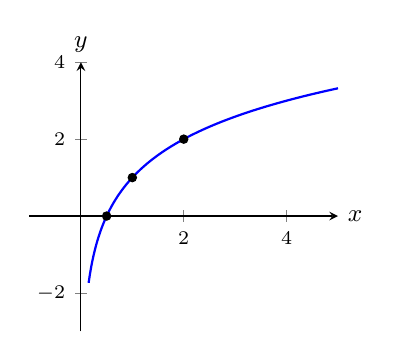
\begin{tikzpicture}
\begin{axis}[myaxis, xmin=-1,xmax=5,ymin=-3,ymax=4]
\addplot[thick,blue,domain=0.15:5]{ln(2*x)/ln(2)};
\addplot[only marks,mark=*,mark size=1.5pt] coordinates {(0.5,0)(1,1)(2,2)};
\end{axis}
\end{tikzpicture}

\textbf{(2)} $y=\log_{2}|x|$：$x>0$ のとき $y=\log_{2}x$，$x<0$ のとき $y=\log_{2}(-x)$．$y$ 軸対称．

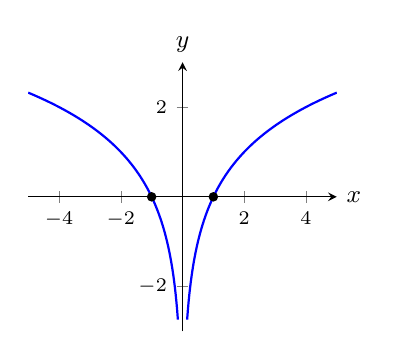
\begin{tikzpicture}
\begin{axis}[myaxis, xmin=-5,xmax=5,ymin=-3,ymax=3]
\addplot[thick,blue,domain=0.15:5]{ln(x)/ln(2)};
\addplot[thick,blue,domain=-5:-0.15]{ln(-x)/ln(2)};
\addplot[only marks,mark=*,mark size=1.5pt] coordinates {(1,0)(-1,0)};
\end{axis}
\end{tikzpicture}
}

\mondai{7}{$a,\;b$ は実数で，$0<a<b<1$ とする．$\log_{a}b+\log_{b}a=\dfrac{8}{3}$ のとき，$\log_{a}b-\log_{b}a$ の値を求めよ．}
\kotae{
$t=\log_{a}b$ とおくと $\log_{b}a=\dfrac{1}{t}$．
\[
t+\dfrac{1}{t}=\dfrac{8}{3}
\]
\[
3t^{2}-8t+3=0 \Rightarrow t=\dfrac{4\pm\sqrt{7}}{3}
\]

$0<a<b<1$ より，底 $a<1$ で真数 $b<1$，しかも $b>a$ なので $0<\log_{a}b<1$．
$\dfrac{4-\sqrt{7}}{3}\approx0.45$ で適．$\dfrac{4+\sqrt{7}}{3}\approx2.22$ は不適．

$t=\dfrac{4-\sqrt{7}}{3},\;\dfrac{1}{t}=\dfrac{4+\sqrt{7}}{3}$．
\[
\log_{a}b-\log_{b}a=t-\dfrac{1}{t}=\dfrac{-2\sqrt{7}}{3}
\]

$\therefore -\dfrac{2\sqrt{7}}{3}$
}

\end{document}
